\documentclass[11pt]{article}
\usepackage{geometry}
\geometry{a4paper, total={6in, 8in}, margin={0in}}
\usepackage{wrapfig}
\usepackage{graphicx}
\usepackage{fullpage}
\usepackage{listings}

\begin{document}

\title{C Project Interim Checkpoint}
\author{Kareem Mehanna, Faraz Malik, Belal Makhzoum, Mohamed Sharif}

\maketitle

\section{Group Organisation and Strategies}

Our group approached the ARM project head-on with the intention of optimising individual workload to maximise productivity. During our first meetings, we decomposed the “Emulator” and assigned specific tasks to each team member using the project management platform, monday.com. We made use of its features to help keep the project on track by managing critical tasks. Each member took ownership of a particular task and split their work into a different file. We defined the headers of each file together so that we could use each other's functions seamlessly and promote code re-usability and modularity. A hierarchical numerical identifier was used to discern between tasks, and also to group related ones, shown with “1.C.2.1” referring to the data processing (immediate) instruction. Our commits refer to these identifiers in order to add important context, while keeping their messages concise. \\
\begin{wrapfigure}{r}{0cm}
\centering
    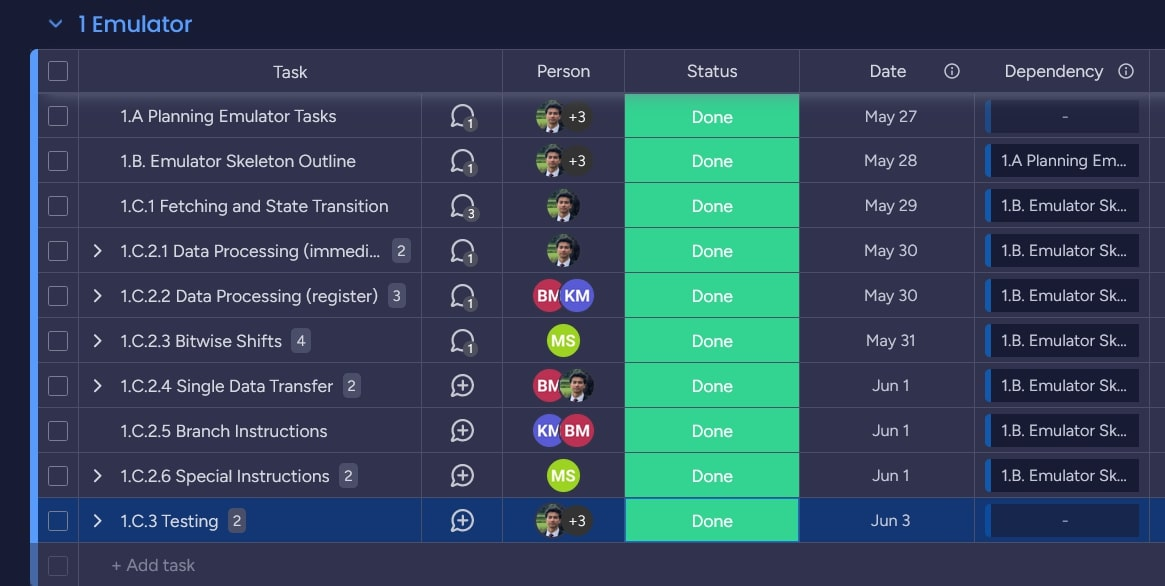
\includegraphics[scale=0.5,width=10cm]{Monday.Com}
    \caption{Using monday.com for allocating “Emulator” tasks.}
\end{wrapfigure}

For the majority of the project, our team decided to fully embrace the benefits of being face-to-face, in the same room. This was a great aid during the debugging stages of the project, given that functions, and their bugs, are best understood by their creators. By leveraging our collective expertise, we rapidly progressed through debugging. To aid collaboration while pair-programming, we made use of CLion's “Code With Me" tool. \\

During planning, we thoroughly digested the specification before constructing a skeleton to provide guidance with splitting the workload. We agreed a standard for function styles and naming conventions. Further modularity was ensured by splitting tasks into different files (linked via Makefile), to minimise development conflicts. \\
\pagebreak
\section{“Emulator” structure}
The decomposition of “Emulator” centered around the following components:
\begin{itemize}
\item  file (input/output)
    \item heap-allocated memory (read/write)
    \item instruction
    \begin{itemize}
        \item decoding
        \item execution (branch, data processing, single data transfer)
    \end{itemize}
\end{itemize}

The processor() procedure decoded the instruction into its main group (i.e. branch), before calling the respective sub-functions to execute different instructions. \\

The “Emulator”'s pipeline mirrored that of an actual processor: fetch, decode, execute. A heap-allocated \lstinline{struct} was used to constantly track the processor's state, with an array of registers,  flags, program counter and the zero register.  \\

During decoding, each instruction was identified, after which it was further deconstructed using bitmasks, after which a series of sub-functions, coupled with utility functions, worked to execute the instruction and update the register's state. \\

As we progress to the “Assembler” task, we fully intend to re-use our existing memory structure to represent the assembled machine code in heap-allocated memory. Thus the reuse of completed functions such as loadData, allocateMemory, etc. will reduce development time, as we intimately understand their operations. However the majority of the assembler will likely be standalone.
\\

\section{Group Performance Review}
As demonstrated by our group successfully completed the testing of “Emulator” by 3 June, we believe that the decision to spend the vast majority of development time in-person has paid off. However, leaving the testing phase at the end of “Emulator” was a taxing decision, and we updated our strategy to incrementally debug throughout the course of development. As a result, we fast-tracked the testing phase of “Assembler”.
\\

Although we were confident with our “Assembler” timeline, we surpassed our expectations by successfully completing its tests today. We did encounter issues with normalising the assembly instructions, and with implementing a tokenizer to be flexible with varying code style, where string manipulation was required. We mitigated this by having granular control of string pointers and heap allocation to prevent segmentation faults. We will use GDB to resolve any remaining problems, and test our code across multiple machines to catch out any architecture-specific errors. Given the difficulty with tracking heap allocation across the “Assembler” source, using leak-detection tools (i.e. Valgrind) should help solve these.

\end{document}
